\section{Market Microstructure}

Market microstructure is the study of the mechanics in place in real markets.
It describes why trading occurs, the mechanics how trades are formed, 
how markets are organized, what information is relayed to the trading 
agents from the markets and the dynamics of price formation. \citep[p. 3-6]{Has07}
In this section we will go through various models how real markets 
are formed and what kinds of elements.

There are several common features with financial markets. They typically are
organized as double auction market 

\subsection{Double Auction}
% Call-market (Itayose, Sealed-bid) vs CDA (Zaraba)

Double auction market is widely used market structure in real 
financial markets. It is a form of auction 
in which both sides of the markets, buyers and sellers, are able to 
produce quotes \citep*{Kle99}. These quotes form the order book 
which is a collection pending bid and ask offers. A trade 
occurs between crossing and matching orders: each trade is formed between 
a bid order with a higher or equal price and an ask order with a lower 
or equal price \citep*{Ben12}. Double auctions varies in
several aspects: when the orders are matched and how the orders are matched. 
In some implementations, such as \citet*{God93}'s, a trade is 
formed only when a buyer and a seller each agree on the exact trade 
price but typically the matching of crossing orders is automated.

% \subsubsection{Order Matching in Double Auction}

Main distinction between double auction market models is when
the order matching takes place. Typically the order matching 
is continuous process occuring after arrival of each new order but
in some markets this process takes place after a specified interval
has passed, for example at the end of a trading day. \citep{boer05}
In literature, there are various terms to describe these two market models
but the mechanics are the same. \citet{boer05} used term 
\textit{call-market} for the former and \textit{continuous session market}
for the latter whereas \citet{ASt05} used terms \textit{Itayose method}
and \textit{Zaraba method} respectively to describe the same mechanics. \citet{Moc15} described
the mechanics of call-markets as \textit{periodic double auction} which
they described is an extension of a sealed-bid auction. Sealed-bid auctions
is an auction model in which the bid and ask offers
are submitted once and then the order matching is executed once. 

% More about Sealed-bid matching (supply-demand) and CDA matching

\subsection{Execution System}
% Quote-driven vs Order-driven
The execution systems are typically divided into two types:
quote-driven and order-driven. In quote-driven market the investors
trade with prices provided by dealers who are part of the market 
organization. In order-driven, the prices are formed according to
the orders submitted by the investors via automatic order matching 
or market makers. \citep{Baru17} Real markets are most often a combination
of the two \citep{boer05}.

\subsection{Price Dynamics}
% Stylized facts
The price dynamics in stock markets are known to be chaotic and hard to 
predict. The underlying elements that play a role in the price formation
are constantly evolving and it still remains relatively poorly understood.
However, there are some characteristics of price behaviour that are supported
with enough empirical evidence to be considered as properties of price in
financial markets. These statistical phenomena, called stylized facts in
econometrics, have been observed in extensive amount of studies from 
different assets, markets and time periods \citep{Shakeel18}. 
% List of Stylized facts (Cont R. (2001) & Gould et al. (2013))
Some of these stylized facts are (\citet{StylizedFacts01} and \citet{lob13}):

\begin{enumerate}
    \item Fat-tailed distribution of returns: distribution of asset returns have fatter tails than normal distribution. Returns have positive excess kurtosis. 
    \par
    \begin{minipage}{\linewidth}
        \centering
        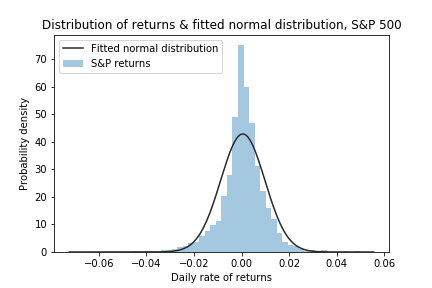
\includegraphics[width=10cm]{plots/S&P500_fat_tails.png}
        \captionof{figure}{Example of fat-tailed of returns}
    \end{minipage}

    \item Lack of autocorrelation: autocorrelation of returns in financial markets have shown to be statistically insignificant except in very short term. Previous return has no prediction power over the following. 
    \par
    \begin{minipage}{\linewidth}
        \centering
        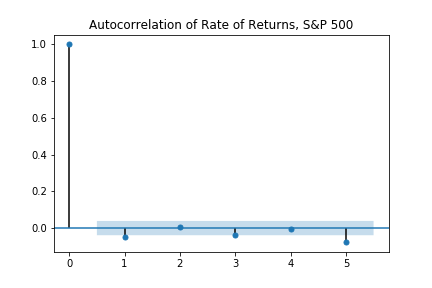
\includegraphics[width=10cm]{plots/S&P500_autocorr.png}
        \captionof{figure}{Example of absense of autocorrelation}
    \end{minipage}

    \item Volatility clusters: volatility have measured to have positive autocorrelation. Strong price movement tend to follow additional exceptional price movements forming clusters of volatility in time.
    \par
    \begin{minipage}{\linewidth}
        \centering
        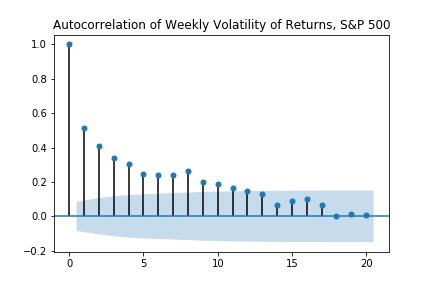
\includegraphics[width=10cm]{plots/S&P500_vola_autocorr.png}
        \captionof{figure}{Example of volatility clustering}
    \end{minipage}
\end{enumerate} 

As has been done in the literature of artificial markets, the representativeness
of the ASM built in this thesis is also validated using these stylized facts.